\newsavebox{\sonorityanglehierarchycompressed}
\savebox{\sonorityanglehierarchycompressed}{
\begin{tikzpicture}[scale=0.8,shorten >=1pt,->]
  \tikzstyle{vertex}=[circle]
  \tikzstyle{point}=[circle,fill=black!25,minimum size=12pt,inner sep=2pt]
  \tikzstyle{line} = [draw, -latex']
  \node[vertex] (RT) at (2.4*8,1)   {RT};
  \node[vertex] (NT) at (2.4*8,0.5)  {NT};
  \node[vertex] (FT) at (2.1*8,1)  {FT};
  \node[vertex] (TT) at (1.4*8,1)     {TT};
  \node[vertex] (RF) at (2.2*8,1)     {RF};
  \node[vertex] (NF) at (2.0*8,1)  {NF};
  \node[vertex] (TF) at (0.6*8,1)   {TF};
  \node[vertex] (FF) at (1.3*8,1)   {FF};
  \node[vertex] (RN) at (1.9*8,1)   {RN};
  \node[vertex] (NN) at (1.2*8,1)   {NN};
  \node[vertex] (FN) at (0.5*8,1)  {FN};
  \node[vertex] (TN) at (0.3*8,1)   {TN};
  \node[vertex] (RR) at (1.1*8,1)  {RR};
  \node[vertex] (NR) at (0.5*8,0.5)  {NR};
  \node[vertex] (FR) at (0.2*8,1)   {FR};
  \node[vertex] (TR) at (0.1*8,1)   {TR};
  \node[vertex] (rising) at (0.3*8,2) {\underline{Rising sonority}};
  \node[vertex] (level) at (1.2*8,2) {\underline{Level sonority}};
  \node[vertex] (falling) at (2.2*8,2) {\underline{Falling sonority}};
  % axis
  \node[vertex] (axisstart) at (-0.23,0) {};
  \node[vertex] (axisend)   at (2.7*8,0) {};
  \draw (axisstart) -- (axisend);
  \draw (0.0*8, 0.2) -- (0.0*8, -0.2) -- cycle;
  \draw (1.0*8, 0.2) -- (1.0*8, -0.2) -- cycle;
  \draw (2.0*8, 0.2) -- (2.0*8, -0.2) -- cycle;
  \node[vertex] (0pointlabel) at (0.0,-0.5) {0};
  \node[vertex] (1pointlabel) at (1.0*8,-0.5) {1};
  \node[vertex] (2pointlabel) at (2.0*8,-0.5) {2};
  \node[vertex] (xaxislabel) at (2.7*8,-0.5) {\textsc{SonAngle}};
\end{tikzpicture}
}

\newsavebox{\sonorityrisehierarchycompressed}
\savebox{\sonorityrisehierarchycompressed}{
\begin{tikzpicture}[scale=0.8,shorten >=1pt,->]
  \tikzstyle{vertex}=[circle]
  \tikzstyle{point}=[circle,fill=black!25,minimum size=12pt,inner sep=2pt]
  \tikzstyle{line} = [draw, -latex']
  \node[vertex] (RT) at (2.5*8, 0)  {RT};
  \node[vertex] (NT) at (1.67*8,0)  {NT};
  \node[vertex] (FT) at (1.25*8,0)  {FT};
  \node[vertex] (TT) at (1*8,-0.5)     {TT};
  \node[vertex] (RF) at (2*8,0)     {RF};
  \node[vertex] (NF) at (1.33*8,-0.5)  {NF};
  \node[vertex] (FF) at (1*8,0)   {FF};
  \node[vertex] (TF) at (0.8*8,-0.5)   {TF};
  \node[vertex] (RN) at (1.5*8,0)   {RN};
  \node[vertex] (NN) at (1*8,0.5)     {NN};
  \node[vertex] (FN) at (0.75*8,0)  {FN};
  \node[vertex] (TN) at (0.6*8,0)   {TN};
  \node[vertex] (RR) at (1*8,1.0)  {RR};
  \node[vertex] (NR) at (0.67*8,-0.5)  {NR};
  \node[vertex] (FR) at (0.5*8,0)   {FR};
  \node[vertex] (TR) at (0.4*8,0)   {TR};
  \node[vertex] (rising) at (0.5*8,2) {\underline{Rising sonority}};
  \node[vertex] (level) at (1*8,2) {\underline{Level sonority}};
  \node[vertex] (falling) at (1.67*8,2) {\underline{Falling sonority}};
  % axis
  \node[vertex] (axisstart) at (-0.23,-1.0) {};
  \node[vertex] (axisend)   at (2.7*8,-1.0) {};
  \draw (axisstart) -- (axisend);
  \draw (0.0*8, -1.2) -- (0.0*8, -0.8) -- cycle;
  \draw (1.0*8, -1.2) -- (1.0*8, -0.8) -- cycle;
  \draw (2.0*8, -1.2) -- (2.0*8, -0.8) -- cycle;
  \node[vertex] (0pointlabel) at (0.0,-1.5) {0};
  \node[vertex] (1pointlabel) at (1.0*8,-1.5) {1};
  \node[vertex] (2pointlabel) at (2.0*8,-1.5) {2};
  \node[vertex] (xaxislabel) at (2.7*8,-1.5) {\textsc{SonRise}};
\end{tikzpicture}
}

\newsavebox{\syllablecontacthierarchy}
\savebox{\syllablecontacthierarchy}{
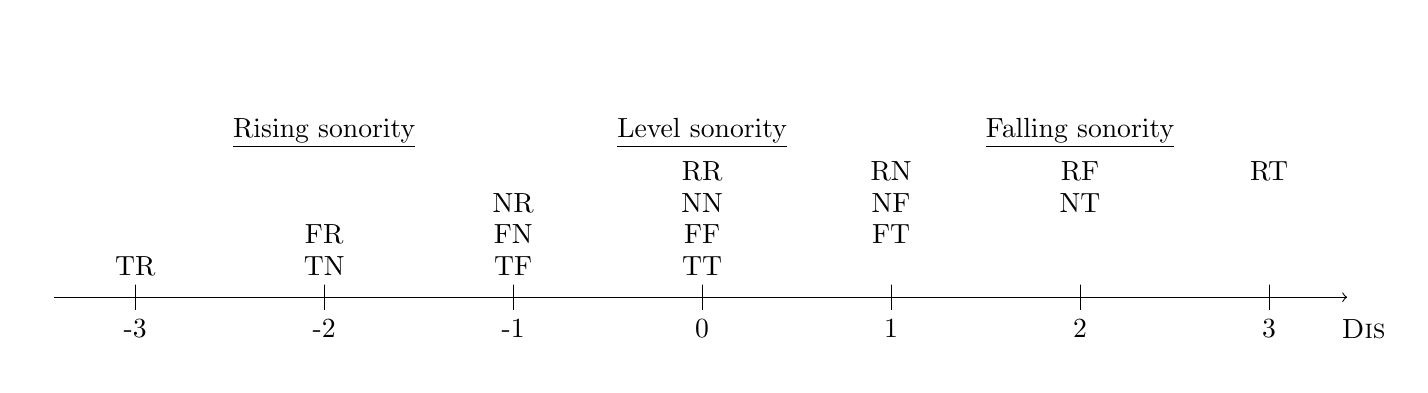
\begin{tikzpicture}[scale=0.8,shorten >=1pt,->]
  \tikzstyle{vertex}=[circle]
  \tikzstyle{point}=[circle,fill=black!25,minimum size=12pt,inner sep=2pt]
  \tikzstyle{line} = [draw, -latex']
  \node[vertex] (RT) at (3*3,2.0)   {RT};
  \node[vertex] (NT) at (2*3,1.5)  {NT};
  \node[vertex] (FT) at (1*3,1.0)  {FT};
  \node[vertex] (TT) at (0*3,0.5)     {TT};
  \node[vertex] (RF) at (2*3,2.0)     {RF};
  \node[vertex] (NF) at (1*3,1.5)  {NF};
  \node[vertex] (FF) at (0*3,1.0)   {FF};
  \node[vertex] (TF) at (-1*3,0.5)   {TF};
  \node[vertex] (RN) at (1*3,2.0)   {RN};
  \node[vertex] (NN) at (0*3,1.5)   {NN};
  \node[vertex] (FN) at (-1*3,1)  {FN};
  \node[vertex] (TN) at (-2*3,0.5)   {TN};
  \node[vertex] (RR) at (0*3,2.0)  {RR};
  \node[vertex] (NR) at (-1*3,1.5)  {NR};
  \node[vertex] (FR) at (-2*3,1.0)   {FR};
  \node[vertex] (TR) at (-3*3,0.5)   {TR};
  % headers
  \node[vertex] (rising) at (2*3,2.6) {\underline{Falling sonority}};
  \node[vertex] (level) at (0*3,2.6) {\underline{Level sonority}};
  \node[vertex] (falling) at (-2*3,2.6) {\underline{Rising sonority}};
  % axis
  \node[vertex] (axisstart) at (-3.5*3,-0) {};
  \node[vertex] (axisend)   at (3.5*3,-0) {};
  \draw (axisstart) -- (axisend);
  \draw (0, 0.2) -- (0, -0.2) -- cycle;
  \draw (1*3, 0.2) -- (1*3, -0.2) -- cycle;
  \draw (2*3, 0.2) -- (2*3, -0.2) -- cycle;
  \draw (3*3, 0.2) -- (3*3, -0.2) -- cycle;
  \draw (-1*3, 0.2) -- (-1*3, -0.2) -- cycle;
  \draw (-2*3, 0.2) -- (-2*3, -0.2) -- cycle;
  \draw (-3*3, 0.2) -- (-3*3, -0.2) -- cycle;
  \node[vertex] (0pointlabel) at (0.0,-0.5) {0};
  \node[vertex] (1pointlabel) at (1.0*3,-0.5) {1};
  \node[vertex] (2pointlabel) at (2.0*3,-0.5) {2};
  \node[vertex] (3pointlabel) at (3.0*3,-0.5) {3};
  \node[vertex] (-1pointlabel) at (-1.0*3,-0.5) {-1};
  \node[vertex] (-2pointlabel) at (-2.0*3,-0.5) {-2};
  \node[vertex] (-3pointlabel) at (-3.0*3,-0.5) {-3};
  \node[vertex] (xaxislabel) at (3.5*3,-0.5) {\textsc{Dis}};
\end{tikzpicture}
}



